% **************************************************
% Document Class Definition
% **************************************************
\documentclass[runningheads]{llncs}

% !TEX root = main.tex
% chktex-file 46

% **************************************************
% Files' Character Encoding
% **************************************************
\PassOptionsToPackage{utf8}{inputenc}
\usepackage{inputenc}
\usepackage[ngerman,english]{babel}

% **************************************************
% Information and Commands for Reuse
% **************************************************
\newcommand{\thesisTitle}{Classification in Big Data Environments}
\newcommand{\thesisName}{Clemens Damke}
\newcommand{\thesisMatNr}{7011488}
\newcommand{\thesisSubject}{Seminar paper}
\newcommand{\thesisDate}{\today}
\newcommand{\thesisVersion}{Draft}

\newcommand{\thesisSupervisor}{Marcel Wever}

\newcommand{\thesisUniversity}{Paderborn University}
\newcommand{\thesisUniversityDepartment}{Department of Computer Science}
\newcommand{\thesisUniversityInstitute}{Heinz Nixdorf Institute}
\newcommand{\thesisUniversityGroup}{Intelligent Systems and Machine Learning Group (ISG)}
\newcommand{\thesisUniversityCity}{Paderborn}
\newcommand{\thesisUniversityStreetAddress}{Warburger Straße 100}
\newcommand{\thesisUniversityPostalCode}{33098}



% **************************************************
% Debug LaTeX Information
% **************************************************
%\listfiles


% **************************************************
% Load and Configure Packages
% **************************************************
\usepackage{geometry}
\geometry{
  a4paper,         % or letterpaper
  textwidth=13cm,  % llncs has 12.2cm
  textheight=23cm, % llncs has 19.3cm
  heightrounded,   % integer number of lines
  hratio=1:1,      % horizontally centered
  vratio=1:1,      % vertically centered
}
\renewcommand{\baselinestretch}{1.15}
\usepackage[parfill]{parskip}

% Colors:
\usepackage[usenames, dvipsnames, svgnames, table]{xcolor}

\definecolor{schwarz}{HTML}{000000}
\definecolor{blau}{HTML}{355FB3}
\definecolor{rot}{HTML}{B33535}
\definecolor{gruen}{HTML}{3BB335}
\definecolor{dunkelblau}{HTML}{1E3666}
\definecolor{hellblau}{HTML}{8ea7d7}

\usepackage{mathtools}
\usepackage{bm}
\usepackage{bbm}
\usepackage{units}
\newcommand\numberthis{\addtocounter{equation}{1}\tag{\theequation}}

\usepackage{algpseudocode}

\usepackage{graphicx}
\usepackage{tikz}
\usetikzlibrary{arrows,positioning}
\usetikzlibrary{calc}
\newcommand{\tikzmark}[1]{\tikz[overlay,remember picture] \node (#1) {};} % chktex 1
\usepackage[labelfont=bf]{caption}
\usepackage{subcaption}

\usepackage{pgfplots}
\usepackage{pgfplotstable}
\pgfplotsset{compat=1.14}
\usepgfplotslibrary{dateplot, statistics}
\pgfplotsset{
    cycle list={blau\\rot\\gruen\\schwarz\\},
}

\usepackage{listings}
\lstset{basicstyle=\ttfamily,breaklines=true}

\usepackage{tasks}
\settasks{counter-format=tsk[1].}

\usepackage[bguq]{frege}
\usepackage{stmaryrd}
\usepackage{multicol}
\usepackage{pbox}
\usepackage{longtable}
\usepackage{booktabs}
\usepackage{csvsimple}
\usepackage{siunitx}

\usepackage{hyperref}
\hypersetup{% setup the hyperref-package options
    pdftitle={\thesisTitle},    %   - title (PDF meta)
    pdfsubject={\thesisSubject},%   - subject (PDF meta)
    pdfauthor={\thesisName},    %   - author (PDF meta)
    plainpages=false,           %   -
    colorlinks=false,           %   - colorize links?
    pdfborder={0 0 0},          %   -
    breaklinks=true,            %   - allow line break inside links
    bookmarksnumbered=true,     %
    bookmarksopen=true          %
}

\usepackage[						% use biblatex for bibliography
	backend=bibtex,					% 	- use biber backend (bibtex replacement) or bibtex
	style=numeric,					% 	- use alphabetic (or numeric) bib style
	natbib=true,					% 	- allow natbib commands
	hyperref=true,					% 	- activate hyperref support
	backref=true,					% 	- activate backrefs
	isbn=false,						% 	- don't show isbn tags
	url=false,						% 	- don't show url tags
	doi=false,						% 	- don't show doi tags
	urldate=long,					% 	- display type for dates
	maxnames=3,%
	minnames=1,%
	maxbibnames=5,%
	minbibnames=3,%
	maxcitenames=2,%
	mincitenames=1%
]{biblatex}
\bibliography{bib-refs}

\makeatletter
\newcounter{rulecount}[section]
\newcommand{\ruleno}[1]{\ensuremath{r_{#1}}}
\newcommand{\rulecurrent}{\ruleno{\therulecount}}
\newcommand{\rulemark}[1]{\refstepcounter{rulecount}(\rulecurrent)\ltx@label{#1}} % chktex 36
\newcommand{\ruleref}[1]{\ruleno{\ref{#1}}}
\makeatother


\newcommand{\Dtrain}{\mathcal{D}_{\mathit{train}}}
\newcommand{\Dvalid}{\mathcal{D}_{\mathit{valid}}}
\newcommand{\Dtest}{\mathcal{D}_{\mathit{test}}}
\newcommand{\sourceinline}[2][source]{{\scriptsize\textsc{#1:~\cite{#2}}}}
\newcommand{\source}[2][source]{\null\hfill\sourceinline[#1]{#2}}

% **************************************************
% Document CONTENT
% **************************************************
\begin{document}

% --------------------------
% Front matter
% --------------------------
% !TEX root = ../main.tex
%

% ------------------------------------  --> main title page
\begin{titlepage}
	\pdfbookmark[0]{Titlepage}{Titlepage}
	\sffamily\

	\begin{figure}
	\begin{minipage}[t]{8.5cm}
	
\includegraphics[height=1.8cm]{gfx/upb_1E}\\
	\textsf{\small{\hspace*{1.3cm}Department of Electrical Engineering,\\
	\hspace*{1.3cm}Computer Science and Mathematics\\
%		\hspace*{1.3cm}Institute of Computer Science\\
		\hspace*{1.3cm}Warburger Straße 100 \\
		\hspace*{1.3cm}33098 Paderborn
		}}
	\end{minipage}
	\hfill
	\begin{minipage}[t]{5cm}
	
\includegraphics[height=1.8cm]{gfx/is-logo-klein}\\
	\textsf{%Institute of Computer Science\\
	\hspace*{0.1cm}\small{Intelligent Systems Group (ISG)}
	}
	\end{minipage}
	\end{figure}

	\centering

	\vfill
	{\large \thesisSubject} \\[5mm]
	{\LARGE \color{ctcolortitle}\textbf{\thesisTitle} \\[10mm]}
	{\Large \thesisName} \\

	\vfill

	\thesisDate\\ % chktex 21

\end{titlepage}


% ------------------------------------  --> lower title back for single page layout
\hfill
\vfill
{
	\small
	\textbf{\thesisName} \\
	\textit{\thesisTitle} \\
	\thesisSubject, \thesisDate\\ % chktex 21
	Supervisor: \thesisSupervisor\\[1.5em] % chktex 21
	\textbf{\thesisUniversity} \\
	\textit{\thesisUniversityGroup} \\
	\thesisUniversityDepartment\\ % chktex 21
	\thesisUniversityStreetAddress\\ % chktex 21
	\thesisUniversityPostalCode\ \thesisUniversityCity\
}

% !TEX root = ../main.tex
%
\begin{abstract}
The training of classifiers on big datasets is an important problem in many domains.
This paper gives an overview of optimization methods that aim to speed up the training process.
We describe two approaches to speed up hyperparameter optimization by learning probabilistic models of error functions.
We then present methods to adapt bootstrapping, gradient descent, logistic regression and SVMs to big datasets.

\keywords{Big Data \and Automated Machine Learning}
\end{abstract}


% --------------------------
% Body matter
% --------------------------


% !TEX root = ../main.tex
\section{Introduction}%
\label{sec:intro}

\pagenumbering{arabic}			% arabic page numbering
\setcounter{page}{1}			% set page counter

Over the last few years Big Data processing has become increasingly important in many domains.
This increase in the data volume also poses new challenges for machine learning applications.
The training time of learners is usually polynomially dependent on the size of the training dataset \(\mathcal{D}_{\mathit{train}}\), i.~e. \(\mathcal{O}(|\mathcal{D}_{\mathit{train}}|^\alpha), \alpha \geq 1\).
Since training has to be repeated for every iteration of cross-validation and hyperparameter search, always using the entire dataset quickly becomes infeasible.
This paper gives an overview of approaches to tackle this problem.

The process of finding an optimal model can in general be split into two phases:
\begin{enumerate}
	\item \textbf{Hyperparameter search:}
		Optimizing a vector \(\lambda\) in the hyperparameter space \(\Lambda_L\) of a learner \(L\) representing a hypothesis space \(\mathcal{H}_{\lambda}\).
		A na\"ive approach to do this is to systematically try configurations using a grid search or a random search over \(\Lambda_L\).
		To evaluate the quality of a given \(\lambda\), \(L\) is usually trained on a training dataset \(\mathcal{D}_{\mathit{train}}\) using \(\lambda\). This yields a hypothesis \(\hat{h}_\lambda \in \mathcal{H}_{\lambda}\) that is evaluated using a validation dataset \(\mathcal{D}_{\mathit{valid}}\).
	\item \textbf{Training or parameter search:}
		Let \(w\) be a vector in the parameter space \(W_{\mathcal{H}_\lambda}\), describing a hypothesis \(h_{\lambda, w} \in \mathcal{H}_\lambda\) given a hyperparameter configuration \(\lambda\).
		The goal of parameter search is to find or approximate a hypothesis \(\hat{h}_\lambda := \arg\min_{h_{\lambda, w}}{e(\mathcal{D}_{\mathit{train}} | h_{\lambda, w})}\), with \(e(\mathcal{D}_{\mathit{train}} | h_{\lambda, w})\) being the empirical error of \(h_{\lambda, w}\) on a given training dataset \(\mathcal{D}_{\mathit{train}}\) according to some error measure.
		Depending on the learner \(L\), various kinds of optimization methods are used to find this minimum, e.~g.\@ bayesian optimization, quadratic programming or, if \(\nabla_w e(\mathcal{D}_{\mathit{train}} | h_{\lambda, w})\) is computable, gradient descent.
		The quality \(f\) of \(\hat{h}_\lambda\) is usually measured by the error on a validation or test dataset, i.~e.\@ \(f(\lambda) := e(\mathcal{D}_{\mathit{valid}} | \hat{h}_\lambda)\).
\end{enumerate}
This paper is structured according to those two phases.
Section \ref{sec:hyperparams} describes ways to speed up the hyperparameter search.
Section \ref{sec:params} then describes how to improve the training methods of existing learners.
Most of the techniques described in this paper improve upon independent components of the model finding process allowing them to be combined.

% !TEX root = ../main.tex
% chktex-file 21
\section{Hyperparameter optimization}%
\label{sec:hyperparams}

As described in the introduction, the goal of hyperparameter optimization is to find a global minimum of \(l\).
Since \(l\) is generally unknown, analytical methods or gradient descent cannot usually be applied.
The only way the get information about \(l\) is to evaluate it, which is costly.
There are multiple ways to reduce the total cost of those evaluations:
\begin{enumerate}
	\item \textbf{Number \(T\) of evaluations of \(l\):}
		During optimization multiple hyperparameter configurations \(\lambda_1, \dots, \lambda_T\) will be evaluated using \(l\).
		\(T\) is usually fixed when using a grid search or a random search.
		After evaluating \(T\) configurations, the best one is chosen.
		Those na{\"\i}ve approaches assume that \(l(\lambda)\) is independent of \(l(\lambda')\) for all pairs \(\lambda \neq \lambda'\).
		We will see that this strong assumption of independence is not necessarily true which in turn allows reducing \(T\).
	\item \textbf{Training dataset size \(S\):}
		The performance of a given configuration \(l(\lambda)\) is computed by training the learner on \(\Dtrain\) which is expensive for big datasets.
		By training on \(S\) instead of \(|\Dtrain|\) datapoints the evaluation can be sped up.
	\item \textbf{Number of training iterations \(E\):}
		Depending on the learner, training often is an iterative process, e.~g.\@ gradient descent.
		To speed up hyperparameter optimization training could be terminated before convergence.
\end{enumerate}

\subsection{FABOLAS}%
\label{sec:hyperparams:fabolas}

The first approach we will discuss is called Fabolas (Fast Bayesian Optimization of Machine Learning Hyperparameters on Large Datasets)~\cite{Klein2016}.
It can be applied to any learner \(L\) and is based upon two main ideas:
\begin{enumerate}
	\item The validation loss \(l\) is modeled as a \textit{Gaussian process} (GP) \(f\) based on the assumption that two configurations \(\lambda\) and \(\lambda'\) will perform similar if they are similar according to some kernel \(k(\lambda, \lambda')\).
		The Gaussian process \(f\) is used as a surrogate to estimate the expected value and variance of \(l\) given \(\lambda\).
		Using \textit{Bayesian optimization} \(l\) will be probed at promising positions to iteratively improve \(f\).
		Hyperparameter configurations that are expected to perform worse than the current optimum will not be probed.
		This effectively reduces \(T\).
	\item The training dataset size \(S\) is modeled as an additional hyperparameter of \(f\) giving the optimizer an additional degree of freedom.
		This allows extrapolating the value of \(l\) when trained on the complete dataset while only probing smaller subsets
		which effectively reduces \(S\).
\end{enumerate}
We will now describe how those two ideas can be applied.

\subsubsection{Gaussian processes}%
\label{sec:hyperparams:fabolas:gaussian}

A Gaussian process is a family of \textit{random variables} (RVs) \({(X_\theta)}_{\theta \in \Theta}\), s.~t.\@ every finite subset of them follows a multivariate normal distribution.
More intuitively it can be understood as a probability distribution over functions \(f: \Theta \to \mathbb{R}\) where \(X_\theta \mathrel{\widehat{=}} f(\theta)\).
Prior knowledge about the likelihood of each \(f\) is described by a prior mean function \(\mu_0(\theta) = \mathbb{E}[f(\theta)]\) and a positive-definite kernel \(k(\theta, \theta') = \mathrm{Cov}(f(\theta), f(\theta'))\).
The covariance kernel models how informative it is to know \(f(\theta)\) to determine \(f(\theta')\).

Let \(\mathcal{D}_n = {\{(\bm{\theta}_i, \bm{y}_i)\}}_{i = 1}^{n}\) denote a set of observations.
Those observations can be used to update the means and variances of the RVs via GP regression.
This collapses the space of possible functions \(f\) to those functions that align with \(\mathcal{D}_n\) (see fig.~\ref{fig:fabolas:matern}):
\begin{align}
	\bm{m} :=&\ {(\mu_0(\bm{\theta}_1), \dots, \mu_0(\bm{\theta}_n))}^T \nonumber \\
	\bm{k}(\theta) :=&\ {(k(\bm{\theta}_1, \theta), \dots, k(\bm{\theta}_n, \theta))}^T \nonumber \\
	\bm{K} \in&\ \mathbb{R}^{n \times n}, \bm{K}_{ij} := k(\bm{\theta}_i, \bm{\theta}_j) \nonumber \\
	\mathbb{E}[f(\theta)\, |\, \mathcal{D}_n] :=&\ \mu_n(\theta) = m_0(\theta) + \bm{k}{(\theta)}^T \bm{K}^{-1} (\bm{y} - \bm{m}) \\
	\mathrm{Cov}(f(\theta), f(\theta')\, |\, \mathcal{D}_n) :=&\ k(\theta, \theta') - \bm{k}{(\theta)}^T \bm{K}^{-1} \bm{k}(\theta')
\end{align}

Fabolas works by modeling the loss function \(l\) as a Gaussian process \(f \sim \mathcal{GP}(m, k)\) with parameter set \(\Theta := \Lambda \times [0, 1]\) where \(\mu_0(\lambda, s) = \mathbb{E}[f(\lambda, s)] = \mathbb{E}[l(\lambda)\, |\, \text{training size}\ s]\).
To model the covariances between different combinations of hyperparameters and training set sizes, the following product kernel is used:
\begin{align}
	k((\lambda, s), (\lambda', s')) :=&\ k_{\textsc{Matérn5}}(d_M(\lambda, \lambda')) \cdot k_{\mathrm{lin}}(s, s')
\end{align}
Here \(k_{\textsc{Matérn5}}\) denotes the stationary Matérn kernel (\(\nu = \nicefrac{5}{2}\)) with \(d_M\) being the Mahalanobis distance between the two compared hyperparameter configurations.
\(k_{\mathrm{lin}}\) essentially is a simple linear kernel modeling the assumption that \(l\) monotonically decreases when \(s\) is increased.
We will now only give an intuition for this choice of kernel and refer to~\citet{Klein2016} for the details.

The Mahalanobis distance \(d_M\) is used instead of the Euclidean distance because the hyperparameters in a configuration typically use very different scales and are in some cases also correlated.
Figure~\ref{fig:fabolas:mahalanobis} gives an intuition for this.
\begin{figure}
	\centering
	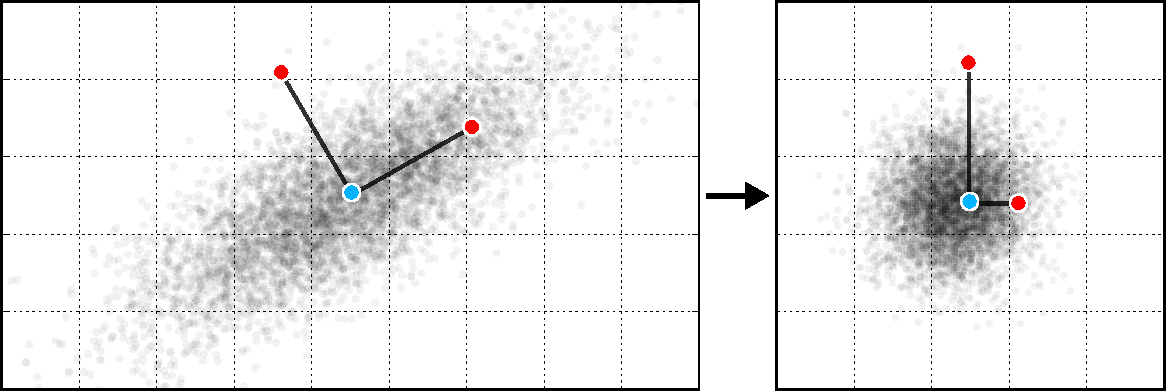
\includegraphics[width=0.75\linewidth]{gfx/fabolas/mahalanobisDistance.pdf}
	\caption{
		Intuition for the Mahalanobis distance.
		Using the Euclidean distance the red points would be equally far away from the blue one.
		The Mahalanobis distance fixes this by first normalizing the hyperparameters and removing correlations.
	}\label{fig:fabolas:mahalanobis}
\end{figure}

Based on the Mahalanobis distance between two configurations \(\lambda, \lambda'\) the \textsc{Matérn5} kernel is used to compute a covariance.
The class of Matérn kernels interpolates between the Gaussian (\textsc{Sq-Exp}) and the exponential (\textsc{Matérn1}) kernel (see fig.~\ref{fig:fabolas:matern}).
Because the exponential kernel drops off quickly, configurations quickly become uncorrelated which causes noisy samples.
The Gaussian kernel drops off less quickly causing smoother samples.
Fabolas uses \textsc{Matérn5} as it empirically fits the smoothness of typical loss functions \(l\) quite well.
\begin{figure}
	\centering
	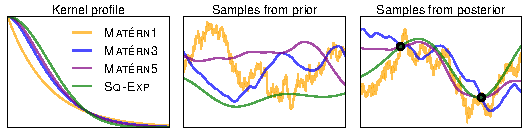
\includegraphics[width=0.75\linewidth]{gfx/fabolas/matern.pdf}
	\caption{
		Comparison between different covariance kernels.
		The middle shows randomly sampled functions \(f\) using different kernels.
		The right shows random samples after two \(f\) values were observed and incorporated into the model via GP regression.
	}\label{fig:fabolas:matern}
\end{figure}

\subsubsection{Bayesian optimization}%
\label{sec:hyperparams:fabolas:bayesian}

To find \(\arg\min_\lambda l(\lambda)\) the bias and variance of \(f\) has to be reduced by probing \(l\) at promising positions.
This is called Bayesian optimization.
The estimated minimum after \(n\) probes is described by \(\arg\min_\lambda \mu_n(\lambda, s = 1)\), i.~e.\@ the configuration with the smallest predicted error on the full test dataset.
To reduce the number of probes required until this minimum converges, an \textit{acquisition function} is used.
Its role is to trade-off exploration vs.\@ exploitation of \(l\) by describing the expected utility of probing \((\lambda_{n+1}, s_{n+1})\) given a set of previous probes \(\mathcal{D}_n\).
Fabolas uses an aquisition function that rates configurations by their \textit{information gain} per computation time:
\begin{align}
	a_F(\lambda, s) :=&\ \frac{1}{c(\lambda, s)} \mathbb{E}_y\left[ p(y\, |\, \lambda, s, \mathcal{D}_n)\ \cdot \mathrm{KL}_{\hat{\lambda}}(p_{\min}(\hat{\lambda}\, |\, \mathcal{D}_n \cup \{(\lambda, s, y)\})\, ||\, u(\hat{\lambda}))\right] \\
	p_{\min}(\lambda\, |\, \mathcal{D}) :=&\ p(\lambda \in \arg\min_{\lambda'}{f(\lambda', s = 1)}\, |\, \mathcal{D}) \nonumber
\end{align}
It measures the expected amount of available information about the optimal configuration if a given configuration were probed, i.~e.\@ the Kullback-Leibler divergence between the density \(p_\min\) of \(\lambda\) being optimal after a probe and the uniform density \(u\).
This information gain of a probe is compared to its expected associated computation time \(c\).
\(c\) is estimated using a separate Gaussian process that is maintained alongside \(f\).
Fabolas considers the cost of a probe because it tries to minimize the total optimization time not the total number of probes.

Since it is infeasible to compute \(a_F\) numerically its maximum is estimated using \textit{Markov-Chain Monte Carlo} (MCMC).
The estimated most promising configuration will be probed.
The resulting loss value and runtime are then used to update the loss model \(f\) and cost model \(c\) via GP regression.

\subsubsection{Evaluation}%
\label{sec:hyperparams:fabolas:eval}
Fabolas was evaluated in \textit{support vector machine} (SVM) and \textit{convolutional neural network} (CNN) optimization tasks on the MNIST and CIFAR-10 dataset respectively.
Figure~\ref{fig:fabolas:eval} compares Fabolas to the following other hyperparameter optimization approaches:
\begin{itemize}
	\item \textbf{Random Search:}
		Simple random hyperparameter search.
		Each configuration is evaluated on the full dataset.
	\item \textbf{Entropy Search \& Expected Improvement:}
		Bayesian optimization methods that always evaluate on the full dataset.
		Expected Improvement uses an aquisition function that simply probes at the current expected optimum.
		Entropy Search uses an aquisition function similar to the one used by Fabolas but without the cost model.
	\item \textbf{MTBO-\(N\) (Multi-Task Bayesian Optimization):}
		Like Fabolas but restricts probes to two sizes \(s \in \{\nicefrac{1}{N}, 1\}\), i.~e.\@ either a small subsample or the entire dataset is used.
		Multiple values for \(N\) were evaluated: 4, 32 and 512.
\end{itemize}
\begin{figure}
	\begin{subfigure}{0.32\textwidth}
		\centering
		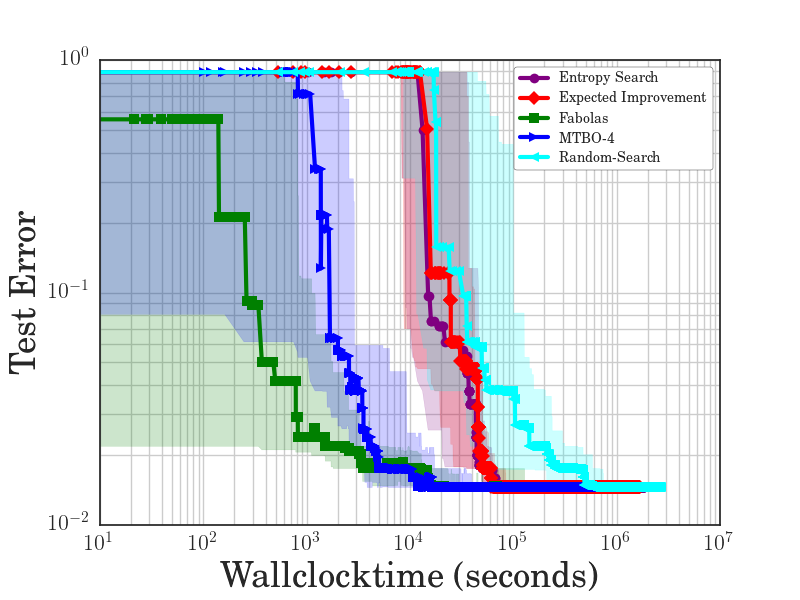
\includegraphics[width=\linewidth]{gfx/fabolas/time1.png}
	\end{subfigure}
	\begin{subfigure}{0.32\textwidth}
		\centering
		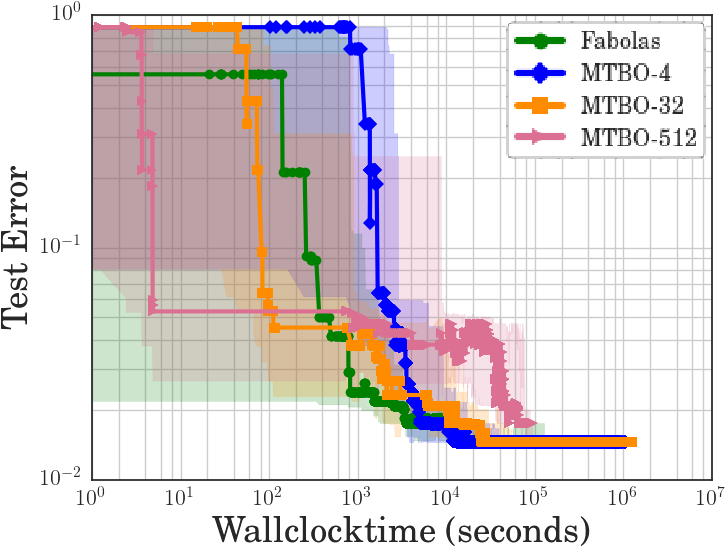
\includegraphics[width=\linewidth]{gfx/fabolas/time2.png}
	\end{subfigure}
	\begin{subfigure}{0.34\textwidth}
		\centering
		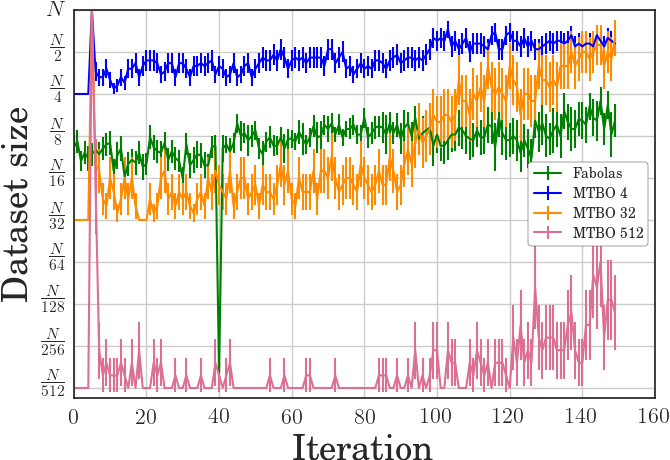
\includegraphics[width=\linewidth]{gfx/fabolas/size.png}
	\end{subfigure}
	\caption{
		SVM optimization on the MNIST dataset.\
		(Left) Comparison of the test performance over time of different optimzers.
		(Middle) Comparison of Fabolas with different MTBO subsample sizes.
		(Right) Comparison of the subsample sizes \(s\) that MTBO and Fabolas choose for their probes.
		The average over 10 runs is depicted.
	}\label{fig:fabolas:eval}
\end{figure}
All Bayesian optimization approaches are at least one order of magnitude faster than random search.
By allowing two probing sizes, MTBO is one additional order of magnitude faster.
Depending on the choice of \(N\) MTBO sometimes improves faster than Fabolas initially.
Once Fabolas starts improving it does however find a good configuration about one order of magnitude faster than MTBO.\
The optimal configuration is found at roughly the same time by both Fabolas and MTBO.\
Overall Fabolas finds a good configuration between 100 and 1000 times faster than random search does.
Similar results are obtained when optimizing CNNs on CIFAR-10.

\subsection{Learning Curve Extrapolation}%
\label{sec:hyperparams:earlyterm}

The second approach for speeding up hyperparameter optimization focuses on reducing the number of training iterations \(E\).
It can in principle be applied to any iterative learner and can be integrated into any hyperparameter optimizer.
The idea is to monitor the learning curve of a learner during training with a hyperparameter configuration \(\lambda\).
If it is unlikely that a good accuracy will be reached with \(\lambda\), training will be terminated before convergence.

The method was first described by \citet{Domhan2015} in the context of hyperparameter optimization for \textit{deep neural networks} (DNNs) that are trained using \textit{stochastic gradient descent} (SGD).

Let \(y_{1:n}\) denote the observed learning curve of SGD after \(n\) iterations, i~e.\@ the sequence of training accuracies \(y_i \in [0, 1]\).
Normally SGD iterations would be run for each hyperparameter configuration \(\lambda\) until convergence or until a maximum number of iterations \(E\) has been reached.
The learning curve extrapolation optimization works by predicting \(y_E\) every \(p\) iterations:
\begin{algorithmic}[1]
\State{\(\hat{y} \gets -\infty\)}
\For{\(\lambda \gets\) next hyperparameter configuration to check}
	\State{\(n \gets 0\)}
	\Repeat\
		\State{Run \(p\) SGD iterations using \(\lambda\) with resulting accuracies \(y_{(n + 1):(n + p)}\).}
		\State{\(n \gets n + p\)}
		\State{Estimate \(P(y_E < \hat{y}\, |\, y_{1:n})\).}\label{line:earlyterm:estimate}
	\Until{\(\text{SGD converged} \lor n \geq E \lor P(y_E < \hat{y}\, |\, y_{1:n}) > \delta\)}
	\State{\algorithmicif\ \(y_n > \hat{y}\) \algorithmicthen\ \(\hat{y} \gets y_n\) \algorithmicend\ \algorithmicif}
\EndFor\
\end{algorithmic}
The prediction step (line~\ref{line:earlyterm:estimate}) uses a probabilistic model.
Similar to Fabolas, a distribution over candidate functions is fit to the observations \(y_{1:n}\).
Unlike Fabolas however, which uses a flexible non-parametric GP model, we use prior knowledge about the shape of learning curves to restrict the model to increasing, saturating functions.
More specifically, the learning curve \(y_{1:n}\) is modeled as a linear combination \(f_{\mathit{comb}}\) of a family of given functions:
\begin{align}
	f_{\mathit{comb}}(t\, |\, \xi) :=&\ \sum_{k = 1}^{K} w_k f_k(t\, |\, \theta_k),\
	\xi = (w_1, \dots, w_k, \theta_1, \dots, \theta_k, \sigma^2) \\
	y_t =&\ f_{\mathit{comb}}(t\, |\, \xi) + \epsilon,\ \epsilon \sim \mathcal{N}(0, \sigma^2)
\end{align}
\citet{Domhan2015} use \(K = 11\) types of functions \(\{f_1, \dots, f_K\}\) that are each parameterized by \(\{\theta_1, \dots, \theta_K\}\).
The assumption is that every function type captures certain aspects of learning curves.
By allowing linear combinations a more powerful model can be obtained.
Figure~\ref{fig:earlyterm:models} illustrates this idea.
\begin{figure}
	\centering
	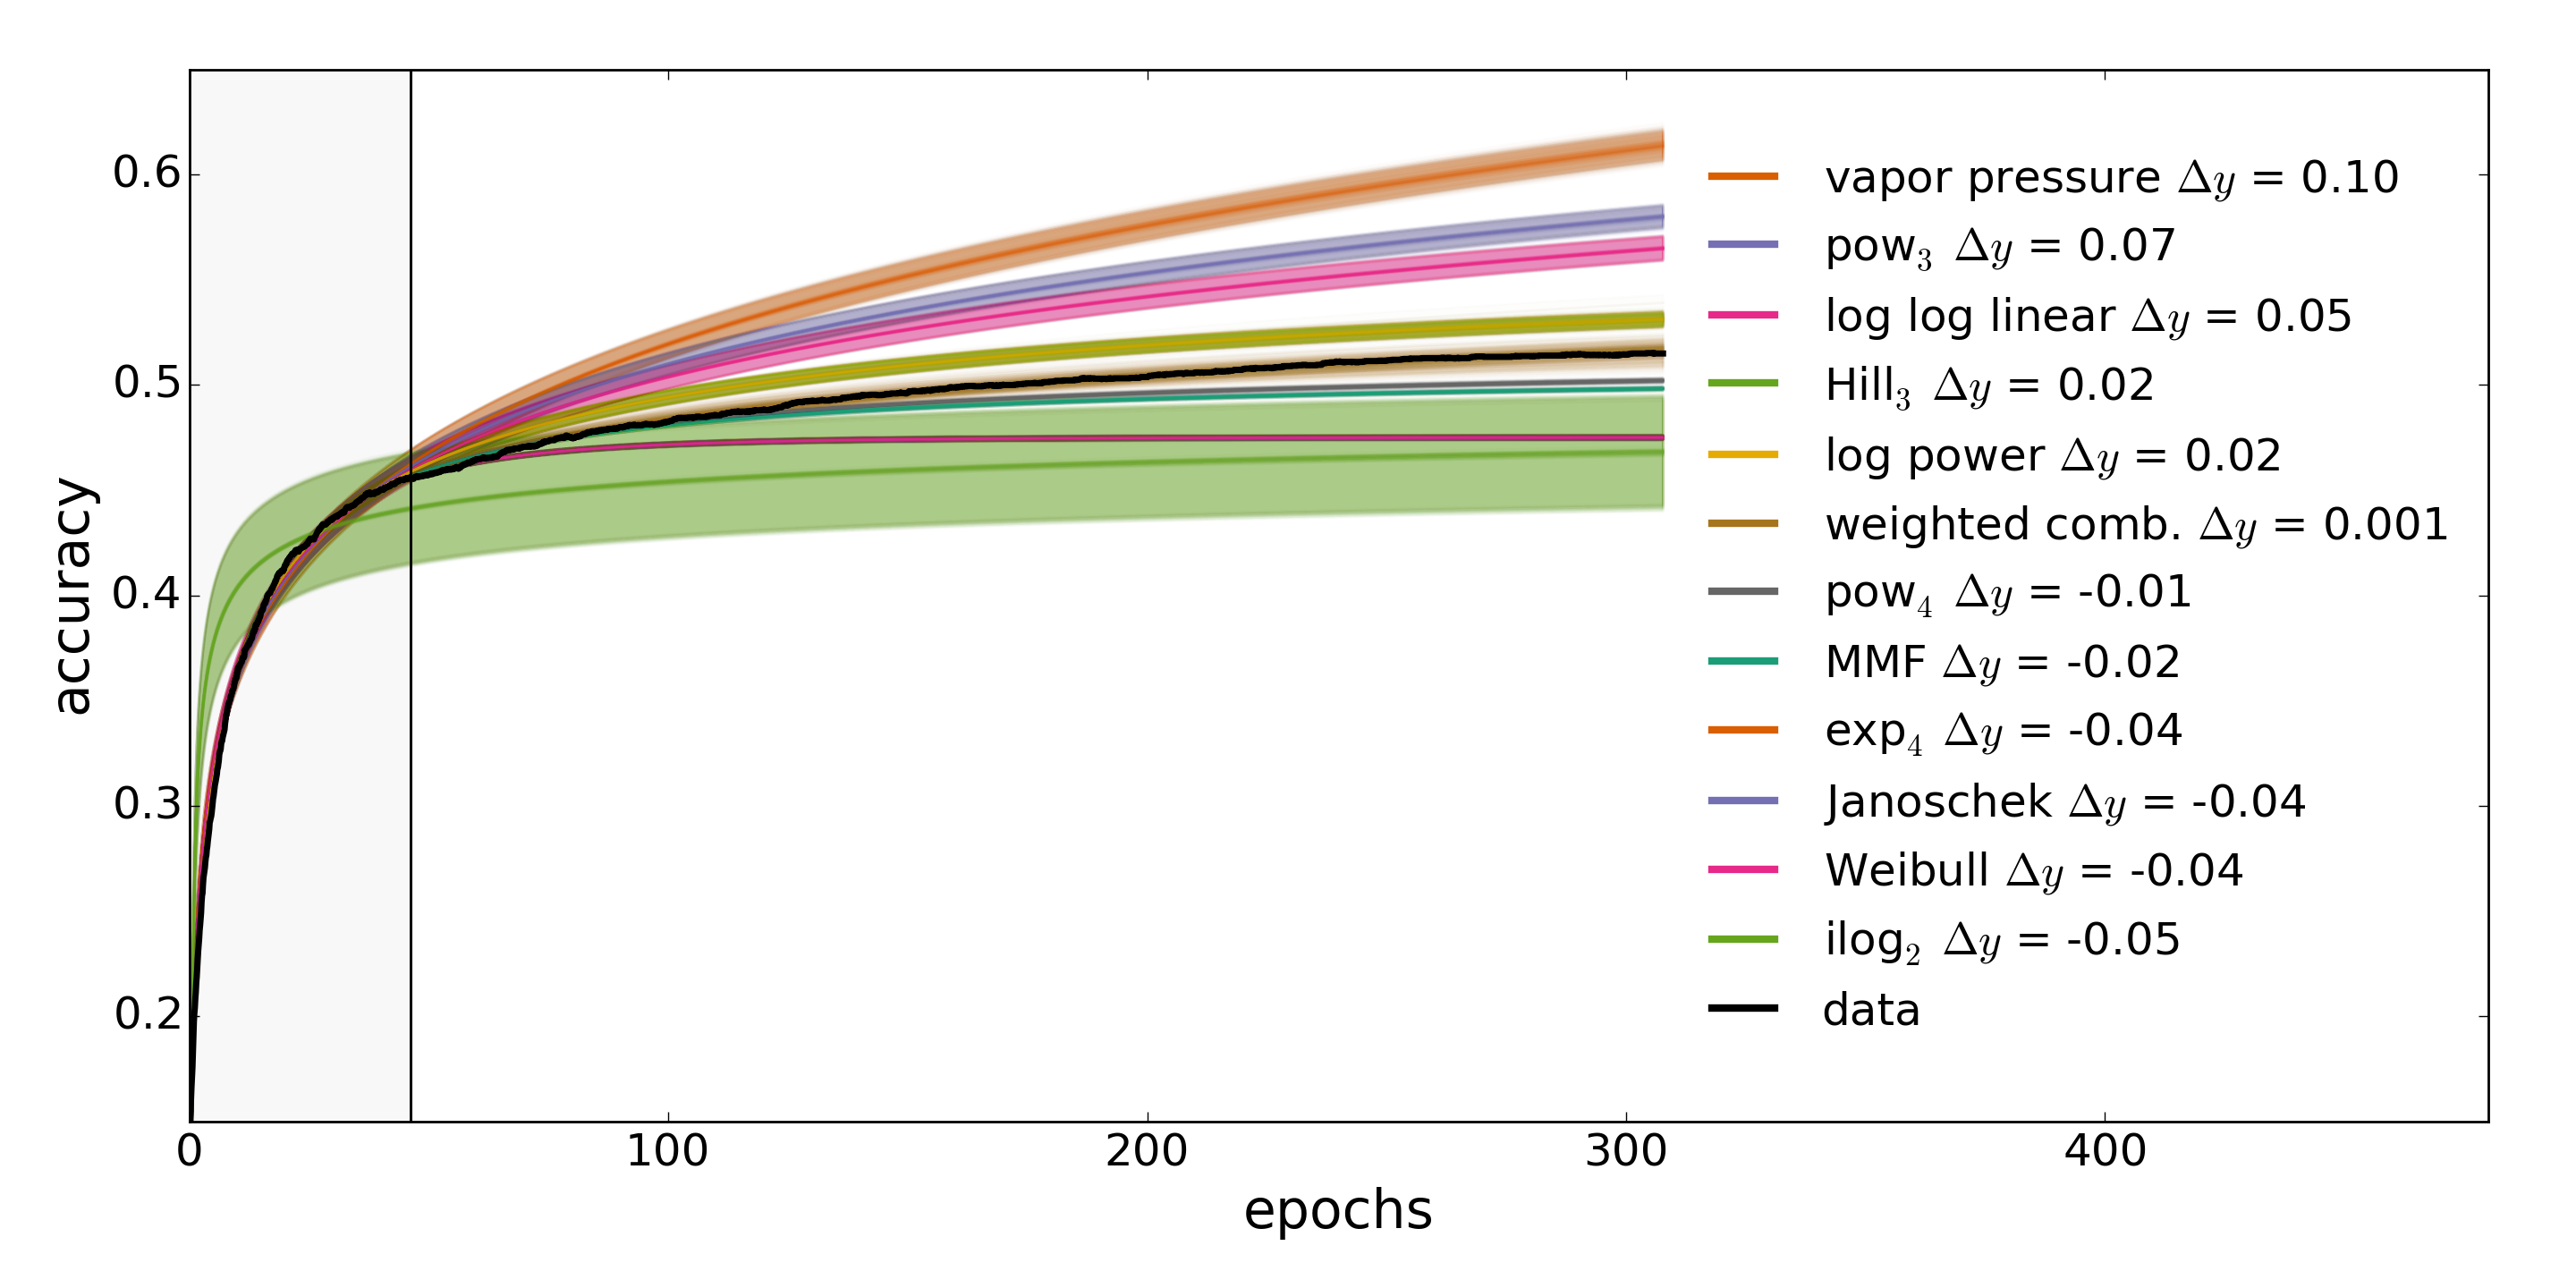
\includegraphics[width=0.75\linewidth]{gfx/earlyterm/models.png}
	\caption{
		Comparison of an observed learning curve (black) with the 11 types of learning curve models and a linear combination of them.
		Each type is parameterized to fit the first 50 observations \(y_{1:50}\).
		As can be seen in the legend on the left, the linear combination has the smallest deviation \(\Delta y\) from the observed data after 300 iterations.
	}\label{fig:earlyterm:models}
\end{figure}

To estimate the probability \(P(y_E < \hat{y}\, |\, y_{1:n})\) MCMC is used to sample \(S\) learning curves \(\{\xi_1, \dots, \xi_S\}\) from the posterior
\begin{align}
	P(\xi\, |\, y_{1:n}) \propto&\ P(y_{1:n}\, |\, \xi) P(\xi) \\
	P(y_{1:n}\, |\, \xi) =&\ \prod_{t = 1}^{n} \mathcal{N}(y_t; f_{\mathit{comb}}(t\, |\, \xi), \sigma^2) \\
	P(\xi) \propto&\ \mathbb{1}[f_{\mathit{comb}}(1\, |\, \xi) < f_{\mathit{comb}}(E\, |\, \xi) \land \forall k: w_k > 0]
\end{align}
The prior on \(\xi\) is used to model the fact that learning curves do not typically decrease over time.
Given the learning curve samples, we can now estimate
\begin{align}
	P(y_E < \hat{y}\, |\, y_{1:n}) =&\ \int P(\xi\, |\, y_{1:n}) P(y_E < \hat{y}\, |\, \xi)\, \mathrm{d}\xi \\
	\approx&\ \frac{1}{S} \sum_{s = 1}^S \Phi(\hat{y}; f_{\mathit{comb}}(E\, |\, \xi_s), \sigma^2) \nonumber
\end{align}

\subsubsection{Evaluation}%
\label{sec:hyperparams:earlyterm:eval}

The early termination method we just described was evaluated on the CIFAR-10, CIFAR-100 and MNIST dataset.
Figure~\ref{fig:earlyterm:eval} shows the behavior of early termination and the obtained speedup on CIFAR-10.
As expected, configurations with learning curves that tend to approach low accuracies are terminated early.
Configurations with high accuracies are run until convergence.
This approach is consistently speeds up the hyperparameter optimization by a factor of two across the tested datasets while reaching the same quality.
\begin{figure}
	\begin{subfigure}{0.4\textwidth}
		\centering
		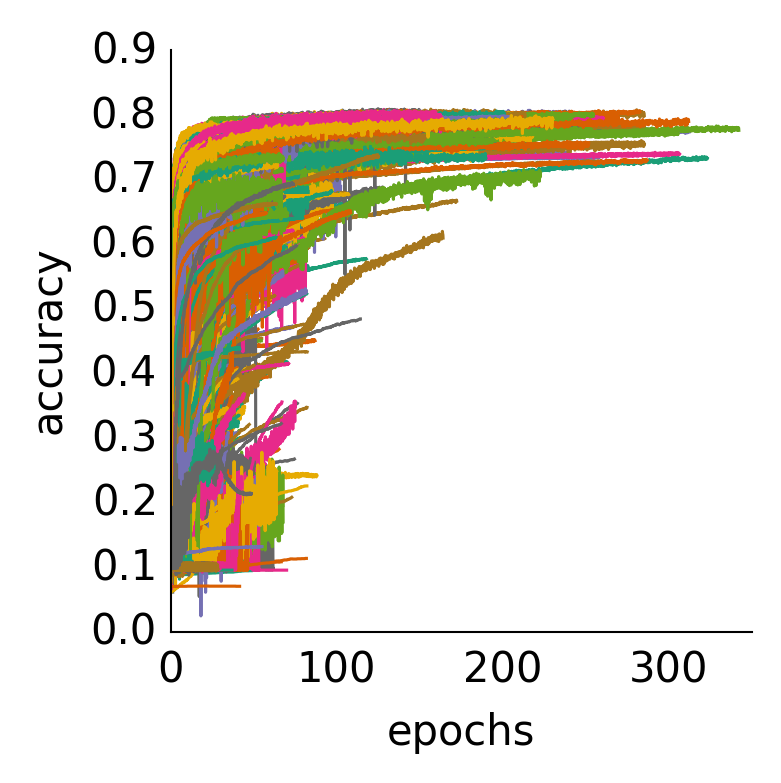
\includegraphics[width=0.9\linewidth]{gfx/earlyterm/samples.png}
	\end{subfigure}
	\begin{subfigure}{0.6\textwidth}
		\centering
		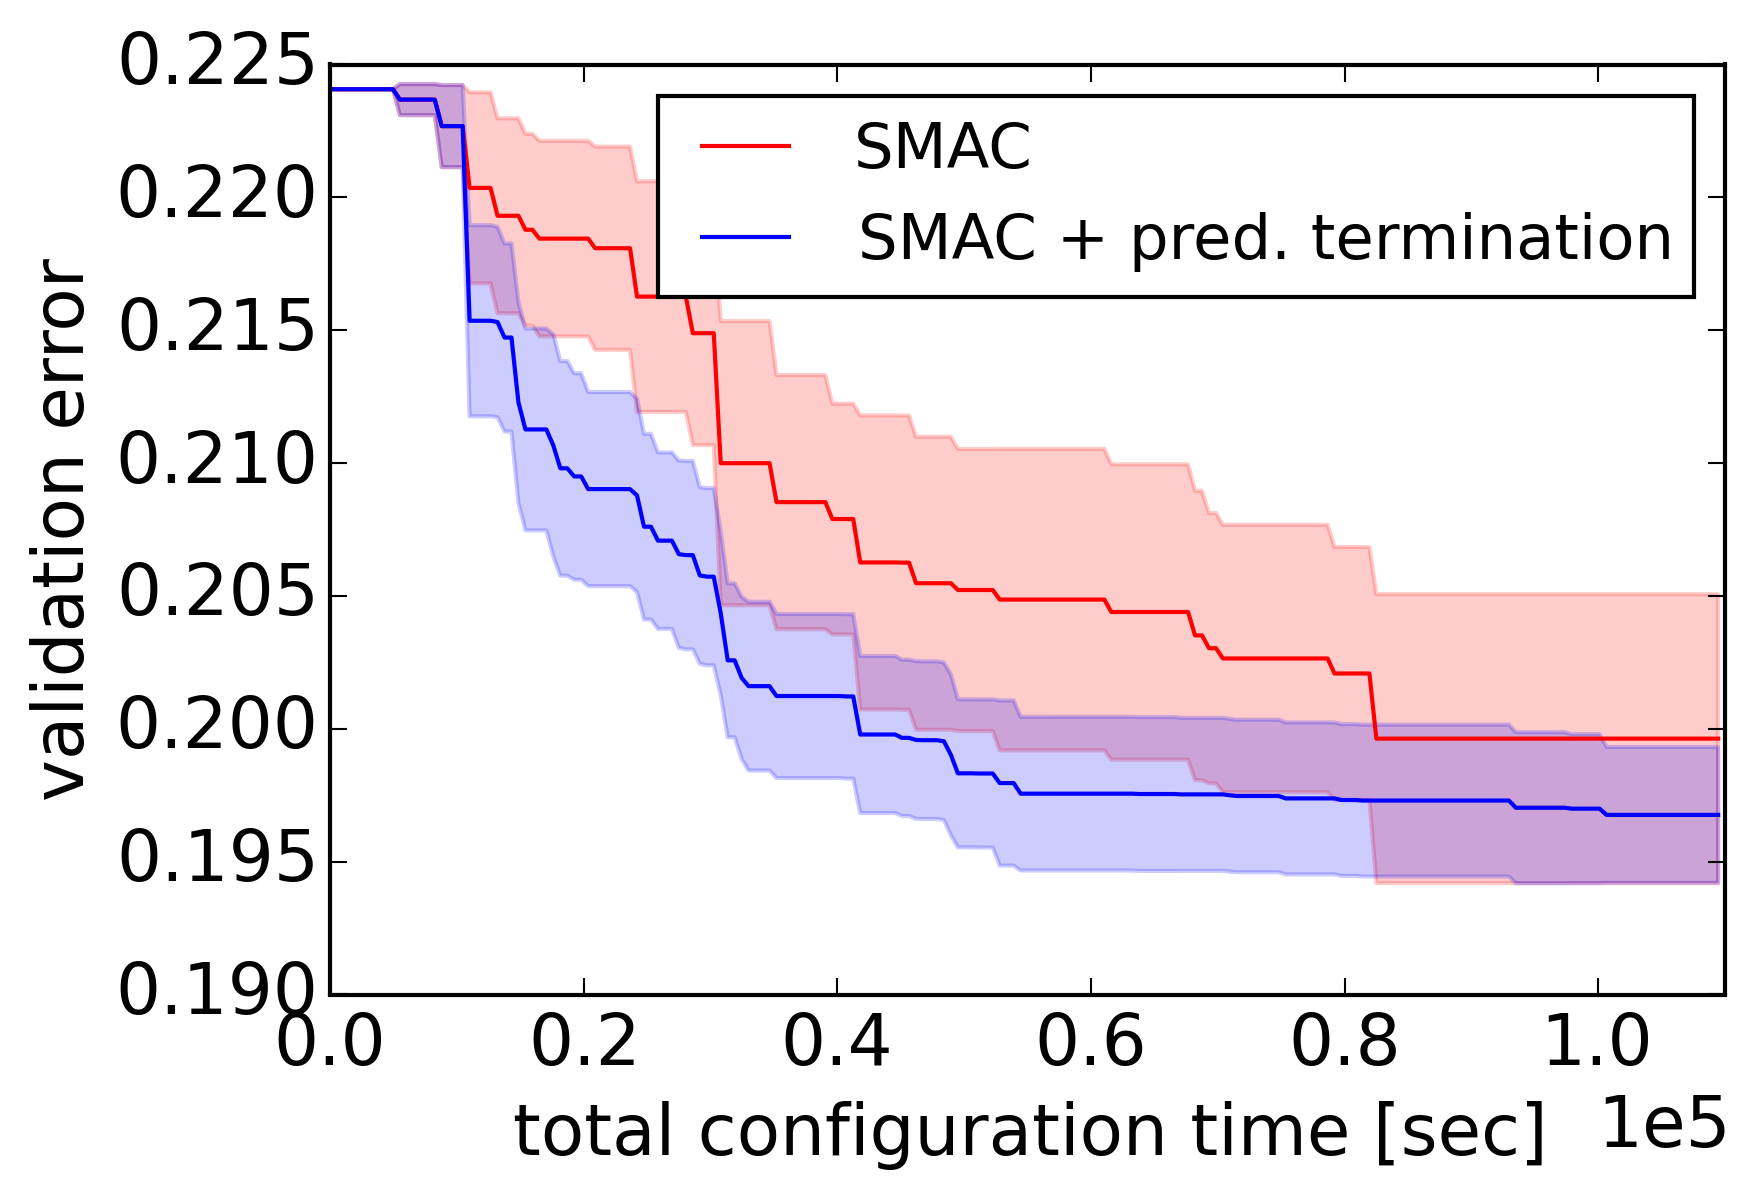
\includegraphics[width=0.85\linewidth]{gfx/earlyterm/time.png}
	\end{subfigure}
	\caption{
		Evaluation on the CIFAR-10 dataset.
		The left graph shows the learning curves of all hyperparameter configurations that were evaluated.
		The right graph shows the average obtained speedup.
	}\label{fig:earlyterm:eval}
\end{figure}

% !TEX root = ../main.tex
% chktex-file 17
% chktex-file 21
\section{Optimizing Training}%
\label{sec:params}

Now follows an overview of approaches to speed up the training process.
We will discuss four approaches:
\begin{enumerate}
	\item A general purpose method that combines subsampling with bootstrapping.
	\item An iterative method to select the optimal subsample size during gradient descent.
	\item Improving the quality of subsampling for logistic regression by weighing the samples.
	\item Speeding up the training of SVMs via \(k\)-means clustering.
\end{enumerate}

\subsection{Bag of Little Bootstraps}%
\label{sec:params:blb}

The first approach we will discuss is called \textit{Bag of Little Bootstraps}~(BLB)~\cite{Kleiner2011}.
It is a bagging method that combines subsampling with bootstrapping and is particularly well suited for parallelized implementations.

In the context of Big Data training typically cannot be performed on the entire dataset.
A na{\"\i}ve way to solve this problem is to simply train on a random \(b\) out of \(n\) subsample of the data \(\Dtrain = \{X_1, \dots, X_n\}\).
This approach is highly sensitive to noise in the training dataset, especially if \(b \ll n\).
To overcome this problem bootstrapping can be used.
The regular \(n\) out of \(n\) bootstrapping technique for variance reduction is not suitable for big datasets because it uses \(63\%\) of the training data on average.
However the \textit{\(b\) out of \(n\) bootstrapping} (BOFN) approach can in principle be applied.
It uses \(s\) samples \(\{\check{X}^{(i)} = (\check{X}_1^{(i)}, \dots, \check{X}_b^{(i)})\, |\, 1 \leq i \leq s\}\) of \(b\) datapoints each.
Since this approach independently learns \(s\) hypotheses \(h_i\) on small datasets \(\check{X}^{(i)}\), their parameterizations \(\theta_i\) tend to have large confidence intervals.
Because of that, the quality of the combined hypothesis is strongly dependent on \(b\)~\cite{Bickel1997}.
BLB reduces this dependence.

\subsubsection{Intuition}%
\label{sec:params:blb:intuition}

\begin{figure}
	\centering
	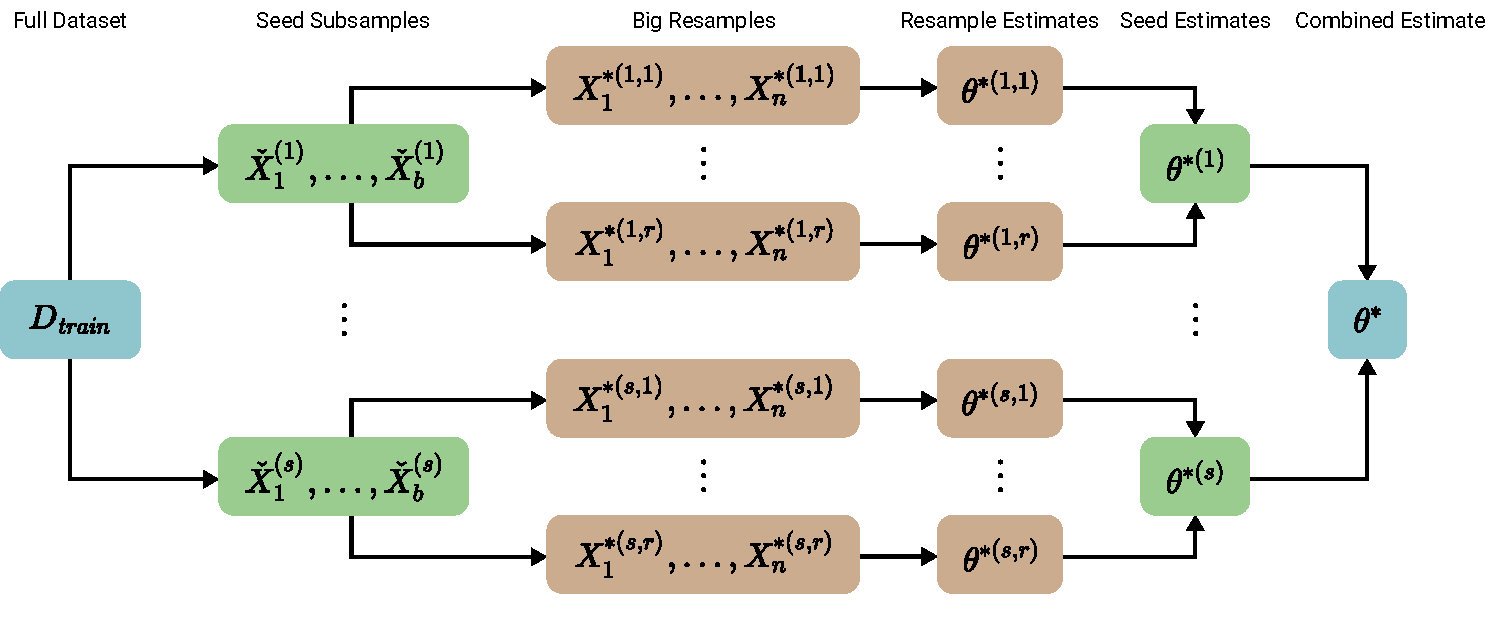
\includegraphics[width=\linewidth]{gfx/blb/overview.pdf}
	\caption{Overview of the steps of BLB.}\label{fig:blb:overview}
\end{figure}
BLB is a simple extension of BOFN that is consistently more robust regarding the choice \(b\) across datasets.
The basic idea is to add another sampling step.
BLB uses each subsample \(\check{X}^{(i)}\) as a seed for \(n\) out of \(b\) sampling.
This yields bigger resamples \(\{X^{*(i, k)} = (X_1^{*(i, k)}, \dots, X_n^{*(i, k)})\, |\, 1 \leq i \leq s, 1 \leq k \leq r\}\) that each contain at most \(b\) different elements.
Training is then run on the resamples \(X^*\) instead of the small seed samples \(\check{X}\).
The learned hypothesis parameterizations are finally combined to a single hypothesis parameterization \(\theta^*\) via a model specific combination function, e.~g.\@ by simply taking the average.
Figure~\ref{fig:blb:overview} illustrates those steps.

Even though BLB trains classifiers on resamples of size \(n\) its time and space complexity effectively still depends on \(b\), not \(n\).
This is because each resample \(X^*\) only contains at most \(b\) different elements which means that it can be efficiently represented by a list of \(b\) multiplicity counts \((c_1, \dots, c_b) \in \mathbb{N}^b\), i.~e.\@ \(\mathit{space} = \mathcal{O}(b \log n)\).
Training on such a dataset is equivalent to training on a dataset of size \(b\) with weights \(w_i = \frac{c_i}{n}\).
Since most commonly used classifiers support weighted samples, BLB is widely applicable.

\subsubsection{Evaluation}%
\label{sec:params:blb:eval}

To show the advantages of BLB for classification it was evaluated with logistic regression on a randomly generated dataset.
Figure~\ref{fig:blb:eval:single} shows that BLB converges on a solution much faster than the regular \(n\) out of \(n\) bootstrapping (BOOT) with comparable results.
It also shows that BLB is less sensitive to the choice of \(b\) than BOFN.\
BLB reached good results with \(b \geq n^{0.6}\) whereas BOFN required at least \(b \geq n^{0.7}\).
\begin{figure}[t]
	\begin{subfigure}[t]{0.66\textwidth}
		\centering
		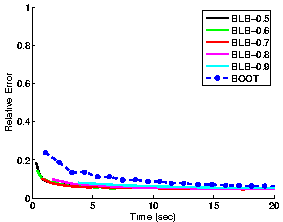
\includegraphics[width=0.49\linewidth]{gfx/blb/time1.pdf}
		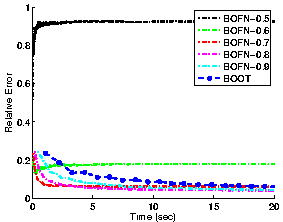
\includegraphics[width=0.49\linewidth]{gfx/blb/time2.pdf}
		\caption{
			Single-threaded results on a subset of the data.
			\(b = n^\gamma\) for multiple values of \(\gamma \in [0.5, 1]\) and \(r = 100\) is used.
			\(s\) is not fixed and grows over time.
		}\label{fig:blb:eval:single}
	\end{subfigure}
	\hfill\
	\begin{subfigure}[t]{0.32\textwidth}
		\centering
		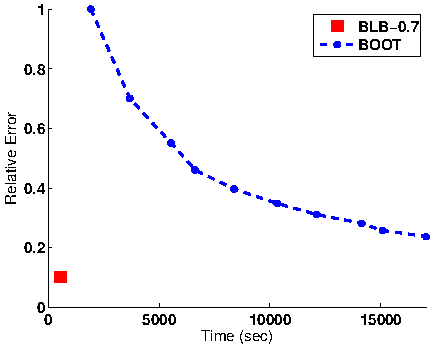
\includegraphics[width=\linewidth]{gfx/blb/parallel.pdf}
		\caption{
			Parallelized results on the entire dataset.
			\(b = n^{0.7}\), \(s = 5\) and \(r = 50\) is used for BLB.\
			For BOOT \(s\) grows over time.
		}\label{fig:blb:eval:parallel}
	\end{subfigure}
	\caption{
		Comparison of BLB and BOFN with BOOT using logistic regression.
		Shows the error on the moving average of all sample hypotheses that are computed within a given time.
		\source{Kleiner2011}
	}\label{fig:blb:eval}
\end{figure}

While BLB already outperforms BOOT without parallelism, as training is overproportionally faster on small samples, its scalability becomes more apparent when parallelized.
Figure~\ref{fig:blb:eval:parallel} shows that BLB significantly outperforms BOOT on a Spark cluster with 10 workers.
This is due to the fact that each BLB sample can be held in memory by its corresponding worker node.
The much larger BOOT samples, on the other hand, require disk reads for large datasets which causes the big difference in runtime.
However even if the BOOT samples are cached in memory, BLB still performs better since training on the compact BLB samples is overproportionally faster than training on regular bootstrap samples.

\subsection{Subsample Size Selection for Gradient Descent}%
\label{sec:params:samplesize}

Next we will discuss an optimization technique for \textit{stochastic gradient descent} (SGD).
The size of the subsample \(\mathcal{S}\) that is considered in a single gradient descent step heavily influences the optimizer's behavior:
\begin{itemize}
	\item In the stochastic approximation regime small samples, typically \(|\mathcal{S}| = 1\), are used. This causes fast but noisy steps.
	\item In the batch regime large samples are used, typically \(|\mathcal{S}| = N\) with \(N := |\Dtrain|\). Steps are expensive to compute but more reliable.
\end{itemize}
Both extremes are usually not suitable for Big Data applications.
Very small samples cannot be parallelized well, making them a bad fit for the compute clusters that are typically available nowadays.
The gradients for very big samples however are often too slow to compute.
\(|\mathcal{S}|\) should ideally lie somewhere in between.

\subsubsection{Size Selection Method}%
\label{sec:params:samplesize:method}

\citet{Byrd2012} describe an iterative algorithm that dynamically increases the size of \(\mathcal{S}\) as long as this promises to significantly reduce the gradient noise.
Let \(\mathcal{S} \subseteq \{1, \dots, N\}\) describe a random subsample of \(\Dtrain = \{(x_i, y_i)\, |\, 1 \leq i \leq N\}\).
SGD will take a step in the descent direction \(d = -\nabla J_{\mathcal{S}}(w)\) where \(J_{\mathcal{S}}(w) := \frac{1}{|\mathcal{S}|} \sum_{i \in \mathcal{S}} \ell(h_{w}(x_i), y_i)\) is the differentiable average loss on \(\mathcal{S}\) given the current configuration \(w\).
Let \(J(w)\) be the average loss on the entire dataset \(\Dtrain\).
\(J(w)\) is the objective function we want to minimize.
Our goal is to trade off \(|\mathcal{S}|\) s.~t.\@ it is as small as possible while \(\nabla J_{\mathcal{S}}(w)\) still \textit{tends to agree} with the objective gradient \(\nabla J(w)\), or more formally
\begin{align}
	\min |\mathcal{S}|\ \text{s.~t.}\ \|\nabla J_{\mathcal{S}}(w) - \nabla J(w) \|_2 \leq \theta \|\nabla J_{\mathcal{S}}(w)\|_2, \theta \in [0, 1)\label{eq:samplesize:cond} % chktex 9
\end{align}
A value of \(\theta = 0\) means that \(\nabla J_{\mathcal{S}}(w)\) always has to be equal to \(\nabla J(w)\),
whereas \(\theta = 1\) would allow steps that directy oppose \(\nabla J(w)\).
Since it is infeasible to compute \(\nabla J(w)\), condition (\ref{eq:samplesize:cond}) can however not be checked directly.
We will instead resort to an estimate and check whether the condition is satisfied in expectation:
\begin{align}
	\underbrace{\mathbb{E}_{\mathcal{S}}[\|\nabla J_{\mathcal{S}}(w) - \nabla J(w) \|_2^2]}_{= \|\mathrm{Var}_{\mathcal{S}}(\nabla J_{\mathcal{S}}(w))\|_1} \leq \theta^2 \|\nabla J_{\mathcal{S}}(w)\|_2^2\label{eq:samplesize:exp}
\end{align}
Computing \(\mathrm{Var}_{\mathcal{S}}(\nabla J_{\mathcal{S}}(w))\) directly is also infeasible because it would require considering all samples of a certain size.
Given a sample \(\mathcal{S}\), the variance of all samples of that size can instead be approximated by
\begin{align}
	\|\mathrm{Var}_{\mathcal{S}}(\nabla J_{\mathcal{S}}(w))\|_1 \approx \frac{1}{|\mathcal{S}| (|\mathcal{S}| - 1)} \sum_{i \in \mathcal{S}} \|\nabla \ell(h_w(x_i), y_i) - \nabla J_{\mathcal{S}}(w)\|_2^2\label{eq:samplesize:approx}
\end{align}
This approximation assumes that \(|\mathcal{S}| \ll N\).
Using (\ref{eq:samplesize:approx}) we can now estimate (\ref{eq:samplesize:exp}) which in turn estimates (\ref{eq:samplesize:cond}).
If we estimate that (\ref{eq:samplesize:exp}) is not satisfied for a given \(\mathcal{S}\), i.~e.\@ that the sample gradient is likely to deviate significantly from the objective gradient, a larger sample \(\widehat{\mathcal{S}}\) has to be used.
In principle we could simply increase the sample size by a constant amount repeatedly and recheck (\ref{eq:samplesize:exp}) but this is slow if \(|\mathcal{S}|\) is far off from satisfying the condition.
Instead we will adaptively choose \(|\widehat{\mathcal{S}}|\) s.~t.\@ it is expected to satisfy (\ref{eq:samplesize:exp}) directly:
\begin{align}
	|\widehat{\mathcal{S}}| = \frac{|\mathcal{S}|\, \|\mathrm{Var}_{\mathcal{S}}(\nabla J_{\mathcal{S}}(w))\|_1}{\theta^2 \|\nabla J_{\mathcal{S}(w)}\|_2^2}\label{eq:samplesize:inc}
\end{align}
Please refer to \citet[chapter~3]{Byrd2012} for a more detailed explanation of (\ref{eq:samplesize:approx}) and (\ref{eq:samplesize:inc}).
To incorporate the ideas described above into the regular SGD algorithm, (\ref{eq:samplesize:exp}) has to be checked after each gradient descent step.
If the check fails, the size of the following samples has to be increased according to (\ref{eq:samplesize:inc}).
Good values for the initial sample size \(|\mathcal{S}_0|\) and for \(\theta\) have to be found via hyperparameter optimization.

The idea outlined above can similarly also be applied to other gradient based optimization methods like the curvature-aware \textit{Newton Conjugate Gradient} (NCG) method.
It not only uses \(\nabla J_{\mathcal{S}}(w)\) but also information from the Hessian \(\nabla^2 J_{\mathcal{S}}(w)\) to compute the direction \(d\) of the next step.
We refer to \citet[chapter~5]{Byrd2012} for the details.

\subsubsection{Evaluation}%
\label{sec:params:samplesize:eval}

Subsample size selection was evaluated on a multi-class logistic regression problem using NCG for optimization.
At first we look at the accuracy of the estimation of (\ref{eq:samplesize:cond}) via (\ref{eq:samplesize:approx}) and (\ref{eq:samplesize:exp}).
On average \(\|\mathrm{Var}_{\mathcal{S}}(\nabla J_{\mathcal{S}}(w))\|_1\) deviates about 4\% from \(\|\nabla J_{\mathcal{S}}(w) - \nabla J(w) \|_2\) on the evaluation dataset if \(|\mathcal{S}| \ll N\)~\cite[tbl.~5.1]{Byrd2012}.

Figure~\ref{fig:samplesize:eval} shows that this accuracy is sufficient.
Dynamic subsample size selection reaches the same quality as the batch method (fixed \(|\mathcal{S}| = N\)) while using significantly fewer datapoints.
This in turn makes it significantly faster.
The speed of convergence however does depend on the choice of \(\theta\).
If \(\theta\) is too small (see \(\theta = 0.1\)), \(|\mathcal{S}|\) is increased quickly which slows down the optimization.
If \(\theta\) is too big (see \(\theta = 0.75\)), \(\nabla J_{\mathcal{S}}(w)\) is allowed to deviate significantly from \(\nabla J(w)\) which causes more erratic gradient steps.
\begin{figure}
	\begin{subfigure}{0.5\textwidth}
		\begin{tikzpicture}
			\begin{axis}[
				width=\linewidth,
				height=0.8\linewidth,
				xmin=0, xmax=6,
				ymin=0.03, ymax=0.14,
				xtick distance=1,
				ytick distance=0.02,
				xlabel={Total Number of Accessed Datapoints \(\times 10^6\)},
				ylabel={Likelihood of \(\Dtrain\)},
				axis x line=bottom,
				axis y line=left,
				label style={font=\tiny},
				tick label style={font=\tiny},
				y tick label style={/pgf/number format/.cd, fixed},
				legend style={
					at={(0.95,0.05)},
					anchor=south east,
					nodes={scale=0.6, transform shape}
				},
				legend cell align={left}
			]
				\addplot table [x=x, y=FG5, col sep=comma] {data/samplesize/performance.csv};
				\addplot table [x=x, y=FG100, col sep=comma] {data/samplesize/performance.csv};
				\addplot table [x=x, y=Dynamic, col sep=comma] {data/samplesize/performance.csv};
				\legend{Fixed \(|\mathcal{S}| = 0.05 N\),Fixed \(|\mathcal{S}| = N\),{Dynamic \(|\mathcal{S}|\), \(\theta = 0.5\)}}
			\end{axis}
		\end{tikzpicture}
	\end{subfigure}
	\begin{subfigure}{0.5\textwidth}
		\begin{tikzpicture}
			\begin{axis}[
				width=\linewidth,
				height=0.8\linewidth,
				xmin=0, xmax=6,
				ymin=0.03, ymax=0.14,
				xtick distance=1,
				ytick distance=0.02,
				xlabel={Total Number of Accessed Datapoints \(\times 10^6\)},
				ylabel={Likelihood of \(\Dtrain\)},
				axis x line=bottom,
				axis y line=left,
				label style={font=\tiny},
				tick label style={font=\tiny},
				y tick label style={/pgf/number format/.cd, fixed},
				legend style={
					at={(0.95,0.05)},
					anchor=south east,
					nodes={scale=0.6, transform shape}
				},
				legend cell align={left}
			]
				\addplot table [x=x, y=10, col sep=comma] {data/samplesize/theta.csv};
				\addplot table [x=x, y=25, col sep=comma] {data/samplesize/theta.csv};
				\addplot table [x=x, y=50, col sep=comma] {data/samplesize/theta.csv};
				\addplot table [x=x, y=75, col sep=comma] {data/samplesize/theta.csv};
				\legend{\(\theta = 0.1\), \(\theta = 0.25\), \(\theta = 0.5\), \(\theta = 0.75\)}
			\end{axis}
		\end{tikzpicture}
	\end{subfigure}
	\caption{
		Results on a multi-class logistic regression task using NCG.\
		(Left) Comparison of dynamic subsample size selection with fixed sample sizes.
		(Right) Comparison of different values for \(\theta\).
		\source[data source]{Byrd2012}
	}\label{fig:samplesize:eval}
\end{figure}

\subsection{Subsampling for Logistic Regression}%
\label{sec:params:osmac}

We will now look at a method that optimizes the subsample selection process for logistic regression.
Subsampling usually increases the \textit{mean squared error} (MSE) of the resulting hypothesis compared to one that is trained on the full dataset \(\Dtrain\).
Let \(\mathcal{S} := \{{(x^*_i, y^*_i)\}}_{i=1}^{r}\) be a random subsample of \(\Dtrain\) that is drawn with or without replacement according to the probabilities \({\{\pi_i\}}_{i=1}^{N}\) where \(N = |\Dtrain|\) and \(\sum_{i=1}^{N} \pi_i = 1\).
Usually \(\mathcal{S}\) is drawn from a uniform distribution, i.~e.\@ each datapoint \(x_i\) is drawn with probability \(\pi_i = N^{-1}\).
Then a \textit{maximum likelihood estimate} (MLE) \(\beta_{\mathcal{S}} = (\beta_{\mathcal{S}}^{(1)}, \dots, \beta_{\mathcal{S}}^{(d)})\) is calculated as an estimate of the objective parameter vector \(\beta_{\Dtrain}\) that maximizes the likelihood of the entire dataset.
This strategy is often not optimal since some data\-points might have a smaller influence on \(\beta_{\Dtrain}\) than others.
The core idea now is to choose the probabilities \(\pi_i\) s.~t.\@ more informative datapoints are more likely to be sampled.

\subsubsection{Case Control}%
\label{sec:params:osmac:cc}

A simple idea to adjust the sampling probabilities \(\pi_i\) is to use \textit{Case-Control subsampling} (CC) in which a roughly equal amount of positive and negative samples is drawn.
Let \(\Dtrain^+ := \{(x, y) \in \Dtrain\, |\, y = 1\}\) and \(\Dtrain^- := \{(x, y) \in \Dtrain\, |\, y = 0\}\).
CC samples would be then chosen without replacement with probabilities
\begin{align}
	\pi_i = \begin{cases}
		|\Dtrain^+|^{-1} & \mathrm{if}\ y_i = 1 \\
		|\Dtrain^-|^{-1} & \mathrm{if}\ y_i = 0
	\end{cases}
\end{align}
This approach however is problematic because it introduces a bias towards unambiguous samples (see fig.~\ref{fig:osmac:cc}).
\begin{figure}
	\centering
	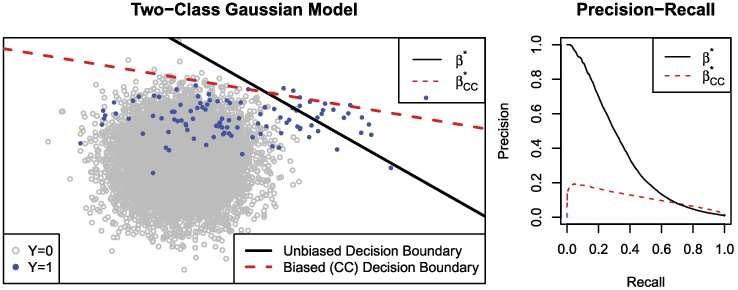
\includegraphics[width=0.7\textwidth]{gfx/osmac/cc.png}
	\caption{Illustration of the bias introduced by CC.\ \sourceinline{Fithian2013}}\label{fig:osmac:cc}
\end{figure}

\subsubsection{Local Case Control}%
\label{sec:params:osmac:lcc}

\citet{Fithian2013} proposed \textit{Local Case-Control subsampling} (LCC) to remove the bias from CC.\
LCC determines the sampling probabilities \(\pi_i\) via a pilot estimate \(\beta_0\).
The estimate \(\beta_0\) is the MLE of a small pilot sample \(\mathcal{S}_0\) that is drawn with uniform or CC sample probabilities.
CC sampling should only be used for the pilot if \(\Dtrain\) contains an imbalanced amount of positive and negative samples.
After determining the pilot estimate \(\beta_0\), datapoints are weighted by the error of the pilot estimator on them:
\begin{align}
	\pi_i = \frac{|y_i - p(x_i\, |\, \beta_0)|}{\sum_{j=1}^{N} |y_j - p(x_j\, |\, \beta_0)|}\
	\mathrm{with}\ p(x\, |\, \beta) = \frac{1}{1 + \exp(\beta^T x)}
\end{align}
Then a bigger sample \(\mathcal{S}_{\mathrm{LCC}}\) is drawn using those probabilities, typically with replacement since this is computationally less expensive.
This produces an estimate \(\beta_{\mathcal{S}_{\mathrm{LCC}}}\) that is consistent with \(\beta_{\Dtrain}\), i.~e.\@ \(\|\beta_{\mathcal{S}_{\mathrm{LCC}}} - \beta_{\Dtrain}\|_2 \to 0\) as \(r \to \infty\).
Additionally LCC prioritizes datapoints that are close to the decision boundary estimated by the pilot.
This tends to reduce the variance of the estimate \(\beta_{\mathcal{S}_{\mathrm{LCC}}}\), especially if \(\Dtrain\) contains an imbalanced amount of positive and negative samples.

\subsubsection{OSMAC}%
\label{sec:params:osmac:idea}

While LCC tends to reduce the estimate's variance, it does not necessarily minimize it.
The \textit{\textbf{O}ptimal \textbf{S}ubsampling \textbf{M}otivated by the \textbf{A}-Optimality \textbf{C}riterion} (OSMAC)~\cite{Wang2018,Wang2017} method improves upon LCC by minimizing the expected variance.\
Like LCC it also uses a pilot estimate \(\beta_0\) but the sampling probabilities \(\pi_i\) are then calculated differently.

Let \(V := \mathrm{Cov}(\beta_{\mathcal{S}} - \beta_{\Dtrain})\) be the covariance matrix of the difference between the sample estimate and the complete dataset estimate.
Given \(\mathbb{E}[\beta_{\mathcal{S}} - \beta_{\Dtrain}] = \mathbf{0}\), \(V\) can be interpreted as a measure of the expected error introduced by subsampling.
Using the A-optimality criterion of optimal design, OSMAC sets the sampling probabilities \(\pi_i\) so that \(\mathrm{tr}(V)\) is minimized in expectation.
More intuitively this minimizes the sum of the MSEs on the regression coefficients \(\beta_{\mathcal{S}}^{(k)}\), i.~e.\@ \(\sum_{k=1}^{d} \mathbb{E}[(\beta_{\mathcal{S}}^{(k)} - \beta_{\Dtrain}^{(k)})^2]\). % chktex 3

It turns out that finding the minimizing probabilities \(\pi_i\) of \(\mathrm{tr}(V)\) is computationally expensive.
However the optimal values for \(\pi_i\) can be approximated using
\begin{align}
	\pi_i = \frac{|y_i - p(x_i\, |\, \beta_0)| \cdot \|x_i\|_2}{\sum_{j=1}^{N} |y_j - p(x_j\, |\, \beta_0)| \cdot \|x_j\|_2}\label{eq:osmac:approx}
\end{align}
The only difference to LCC here is the added \(\|x_i\|_2\) factor.
The intuition behind this is that samples with large norms tend to be further away from the decision boundary%
\footnote{
	This intuition is not entirely correct since it does not consider the offset and rotation of the decision boundary.
	Those aspects are ignored because (\ref{eq:osmac:approx}) only approximates the A-optimal probabilities.
	For details please refer to \citet[chapter 3.2]{Wang2017}.
}.
An incorrectly classified sample that is far from the decision boundary is more surprising than an incorrectly classified sample close to it.
Since the sigmoidal \(p\) function saturates quickly this fact is often not captured by LCC sampling.

\subsubsection{Evaluation}%
\label{sec:params:osmac:eval}

We will now compare uniform, LCC and OSMAC sampling on two datasets.
The datapoints \(x_i\) are randomly sampled from different distributions.
The corresponding classes \(y_i \in \{0, 1\}\) are then assigned using a fixed coefficient vector \(\beta\).
These two datasets are used:
\begin{itemize}
	\item \textbf{mzNormal:}
		Uses a multivariate normal distribution \(\mathcal{N}(0, \Sigma)\) with mean \(0\) and \(\Sigma_{i j} = 0.5^{\delta_{i \neq j}}\).
		Contains a roughly equal amount of positive and negative samples.
	\item \textbf{nzNormal:}
		Uses a multivariate normal distribution \(\mathcal{N}(1.5, \Sigma)\) with mean \(1.5\).
		About 95\% of the samples are positive.
\end{itemize}

Figure~\ref{fig:osmac:mse} shows the MSEs \(\|\beta_{\mathcal{S}} - \beta\|_2^2\) for different subsample sizes \(r\).
OSMAC consistently gives the closest approximation of \(\beta\), confirming its theoretical A-optimality.
The reduced coefficient approximation error in turn results in a reduced error of \mbox{OSMAC} on \(\Dtrain\).
\begin{figure}[t]
	\begin{subfigure}{0.5\textwidth}
		\begin{tikzpicture}
			\begin{axis}[
				width=\linewidth,
				height=0.8\linewidth,
				xmin=100, xmax=1000,
				ymin=0, ymax=0.8,
				xtick distance=200,
				ytick distance=0.2,
				xlabel={\(r\)},
				ylabel={MSE},
				axis x line=bottom,
				axis y line=left,
				label style={font=\tiny},
				tick label style={font=\tiny},
				y tick label style={/pgf/number format/.cd, fixed},
				legend style={
					at={(0.95,0.95)},
					anchor=north east,
					nodes={scale=0.6, transform shape}
				},
				legend cell align={left}
			]
				\addplot table [x=x, y=uniform, col sep=comma] {data/osmac/mse-mzNormal.csv};
				\addplot table [x=x, y=LCC, col sep=comma] {data/osmac/mse-mzNormal.csv};
				\addplot table [x=x, y=OSMAC, col sep=comma] {data/osmac/mse-mzNormal.csv};
				\addplot [dashed] table [x=x, y=full, col sep=comma] {data/osmac/mse-mzNormal.csv};
				\legend{uniform, LCC, OSMAC, full}
			\end{axis}
		\end{tikzpicture}
		\caption{mzNormal}
	\end{subfigure}
	\begin{subfigure}{0.5\textwidth}
		\begin{tikzpicture}
			\begin{axis}[
				width=\linewidth,
				height=0.8\linewidth,
				xmin=100, xmax=1000,
				ymin=0, ymax=2.5,
				xtick distance=200,
				ytick distance=0.5,
				xlabel={\(r\)},
				ylabel={MSE},
				axis x line=bottom,
				axis y line=left,
				label style={font=\tiny},
				tick label style={font=\tiny},
				y tick label style={/pgf/number format/.cd, fixed},
				legend style={
					at={(0.95,0.95)},
					anchor=north east,
					nodes={scale=0.6, transform shape}
				},
				legend cell align={left}
			]
				\addplot table [x=x, y=uniform, col sep=comma] {data/osmac/mse-nzNormal.csv};
				\addplot table [x=x, y=LCC, col sep=comma] {data/osmac/mse-nzNormal.csv};
				\addplot table [x=x, y=OSMAC, col sep=comma] {data/osmac/mse-nzNormal.csv};
				\addplot [dashed] table [x=x, y=full, col sep=comma] {data/osmac/mse-nzNormal.csv};
				\legend{uniform, LCC, OSMAC, full}
			\end{axis}
		\end{tikzpicture}
		\caption{nzNormal}
	\end{subfigure}
	\caption{MSEs on \(\beta\) for different subsample sizes \(r\). \sourceinline[data source]{Wang2017}}\label{fig:osmac:mse}
\end{figure}

\subsection{Clustering for SVMs}%
\label{sec:params:wkmsvm}

To speed up the training of SVMs \citet{Almeida2000} proposed a simple method that reduces the dataset size via \(k\)-means clustering.
It can be described as a simple three-step procedure:
\begin{enumerate}
	\item Group the training samples \(\Dtrain\) into \(k\) clusters \(C_1, \dots, C_k\) with centers \(c_1, \dots, c_k\) where \(k\) should be determined via hyperparameter optimization.
	\item Check for each cluster \(C_i\) whether all associated datapoints belong to the same class, i.~e.\@ \(\exists\, z \in \{+1, -1\}: \forall (x, y) \in C_i: y = z\).
		If yes, all datapoints in \(C_i\) are removed from \(\Dtrain\) and replaced by \(c_i\).
		If not, they are kept in the dataset.
		The intuition behind this is that clusters with points from multiple classes might be near the decision boundary so they are kept to serve as potential support vectors.
	\item Finally standard SVM training is performed on the reduced training dataset.
\end{enumerate}
This approach performs similarly to SVM training on the full dataset.
However the size of the reduced dataset is very unpredictable.
Large homogeneous clusters with only a few noisy outliers of a different class will not be used to reduce the dataset size.
Because of that the effective speedup and memory requirements may vary greatly depending on the dataset.

\citet{Lee2007} proposed KM-SVM, an alternative approach that solves this problem by performing clustering on the datapoints of each class separately.
This method has more predictable time and memory requirements but it also tends to modify the structure of the dataset.
Figure~\ref{fig:wkmsvm:compare:km} shows that this can cause KM-SVM to deviate significantly from the full dataset SVM.\
\begin{figure}
	\begin{subfigure}{0.5\textwidth}
		\centering
		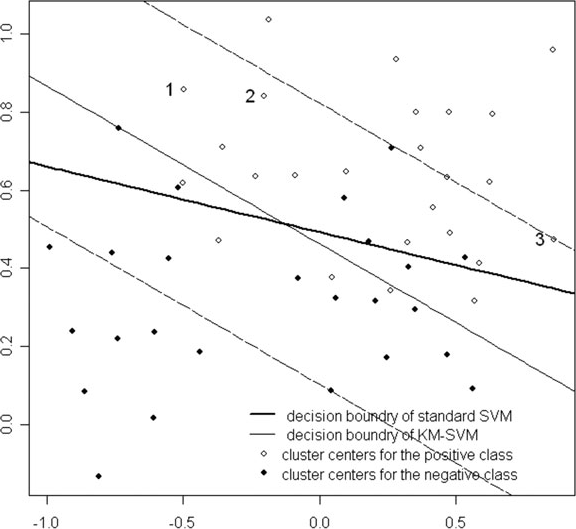
\includegraphics[width=0.85\linewidth]{gfx/wkmsvm/km.png}
		\caption{KM-SVM}\label{fig:wkmsvm:compare:km}
	\end{subfigure}
	\begin{subfigure}{0.5\textwidth}
		\centering
		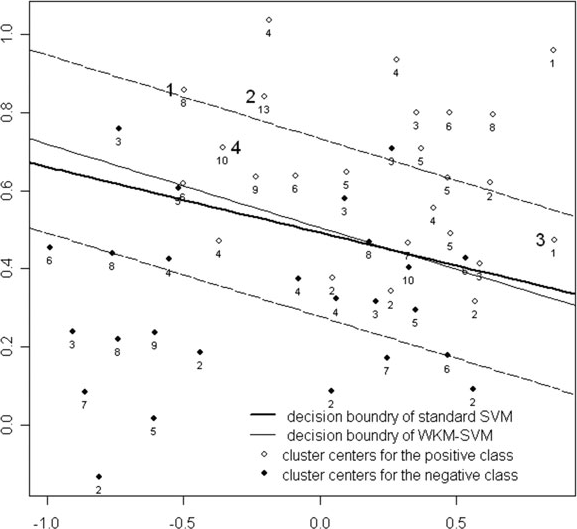
\includegraphics[width=0.85\linewidth]{gfx/wkmsvm/wkm.png}
		\caption{WKM-SVM}\label{fig:wkmsvm:compare:wkm}
	\end{subfigure}
	\caption{
		Comparison of the decision boundaries of KM-SVM and WKM-SVM.\
		The numbers next to the cluster centers on the right represent the cluster weights.
		\source{Bang2014}
	}\label{fig:wkmsvm:compare}
\end{figure}

WKM-SVM~\cite{Bang2014} improves upon KM-SVM by weighting each cluster center \(c_i\) by the amount of datapoints \(|C_i|\) it represents.
This solves the problem that small clusters of outliers have the same influence on the decision boundary as big clusters of more representative datapoints in KM-SVM.\
Figure~\ref{fig:wkmsvm:compare:wkm} shows how this improves the quality of the decision boundary.

\subsubsection{Evaluation}%
\label{sec:params:wkmsvm:eval}

We will now compare KM-SVM and WKM-SVM using different compression rates \(R \in \{1, 3, 5, 10\}\) that describe the number of clusters \(k = \frac{|\Dtrain|}{R}\).
A compression rate of \(R = 1\) corresponds to a SVM that is trained on the entire dataset.
For \(\Dtrain\) the \texttt{PimaIndiansDiabetes2} dataset is used.
Figure~\ref{fig:wkmsvm:eval} shows that WKM-SVM consistently performs better than KM-SVM with a roughly identical training time.
Both clustering methods improve the runtime significantly without any significant increases in the test error.
\begin{figure}[t]
	\begin{subfigure}{0.33\textwidth}
		\begin{tikzpicture}
			\begin{axis}[
				width=\linewidth,
				height=0.8\linewidth,
				xmin=1, xmax=10,
				ymin=0, ymax=0.3,
				xtick={1,3,5,10},
				ytick distance=0.05,
				xlabel={\(R\)},
				ylabel={Test error},
				axis x line=bottom,
				axis y line=left,
				label style={font=\tiny},
				tick label style={font=\tiny},
				y tick label style={/pgf/number format/.cd, fixed},
				legend style={
					at={(0.95,0.05)},
					anchor=south east,
					nodes={scale=0.6, transform shape}
				},
				legend cell align={left}
			]
				\addplot table [x=compression, y=km-err, col sep=comma] {data/wkmsvm/diabetes.csv};
				\addplot table [x=compression, y=wkm-err, col sep=comma] {data/wkmsvm/diabetes.csv};
				\legend{KM, WKM}
			\end{axis}
		\end{tikzpicture}
	\end{subfigure}
	\begin{subfigure}{0.33\textwidth}
		\begin{tikzpicture}
			\begin{axis}[
				width=\linewidth,
				height=0.8\linewidth,
				xmin=1, xmax=10,
				ymin=0, ymax=1250,
				xtick={1,3,5,10},
				ytick distance=200,
				xlabel={\(R\)},
				ylabel={Training time (sec)},
				axis x line=bottom,
				axis y line=left,
				label style={font=\tiny},
				tick label style={font=\tiny},
				y tick label style={/pgf/number format/.cd, fixed},
				legend style={
					at={(0.95,0.95)},
					anchor=north east,
					nodes={scale=0.6, transform shape}
				},
				legend cell align={left}
			]
				\addplot table [x=compression, y=km-time, col sep=comma] {data/wkmsvm/diabetes.csv};
				\addplot table [x=compression, y=wkm-time, col sep=comma] {data/wkmsvm/diabetes.csv};
				\legend{KM, WKM}
			\end{axis}
		\end{tikzpicture}
	\end{subfigure}
	\begin{subfigure}{0.32\textwidth}
		\begin{tikzpicture}
			\begin{axis}[
				width=\linewidth,
				height=0.8\linewidth,
				xmin=1, xmax=10,
				ymin=0, ymax=185,
				xtick={1,3,5,10},
				ytick distance=25,
				xlabel={\(R\)},
				ylabel={Support vectors},
				axis x line=bottom,
				axis y line=left,
				label style={font=\tiny},
				tick label style={font=\tiny},
				y tick label style={/pgf/number format/.cd, fixed},
				legend style={
					at={(0.95,0.95)},
					anchor=north east,
					nodes={scale=0.6, transform shape}
				},
				legend cell align={left}
			]
				\addplot table [x=compression, y=km-sv, col sep=comma] {data/wkmsvm/diabetes.csv};
				\addplot table [x=compression, y=wkm-sv, col sep=comma] {data/wkmsvm/diabetes.csv};
				\legend{KM, WKM}
			\end{axis}
		\end{tikzpicture}
	\end{subfigure}
	\caption{Comparison of KM-SVM and WKM-SVM.\ \sourceinline[data source]{Bang2014}}\label{fig:wkmsvm:eval}
\end{figure}

% !TEX root = ../main.tex
% chktex-file 21
\section{Conclusion}%
\label{sec:conclusion}

In this paper we presented two approaches to speed up hyperparameter optimization: Fabolas and learning curve extrapolation.
Both use probabilistic models to estimate values of the error function.
Then four approaches to speed up training were presented: Bag of Little Bootstraps, subsample size selection for gradient descent, subsampling for logistic regression and \(k\)-means clustering for SVMs.\
All presented approaches are able to speedup training significantly on big datasets.
Since those approaches optimize different aspects of the training process, various combinations of them are possible to get further speedups.
We will now take a brief look at promising combinations:
\begin{itemize}
	\item Since Fabolas is a hyperparameter optimizer that does not make assumptions about the learner, it can be combined trivially with any of the training optimization approaches presented in Section~\ref{sec:params}.
	\item The learning curve extrapolation method described in Section~\ref{sec:hyperparams:earlyterm} requires a learner using gradient descent.
		It can thus be combined with the subsample size selection method described in Section~\ref{sec:params:samplesize}.
	\item Learning curve extrapolation could additionally be combined with Fabolas to guide the hyperparameter search.
		This would however require changing the covariance kernel of the cost model \(c\) since probes at suboptimal positions are likely to be terminated early, making them less costly and thus more attractive for the aquisition function \(a_F\).
		One possible approach to adapt the cost model is to add a dependence on the loss model \(f\).
		This would essentially merge the two Gaussian processes \(c\) and \(f\) into a single cost-loss model over the parameter space \(\Theta = \Lambda \times [0, 1] \times \{\mathrm{cost}, \mathrm{loss}\}\) where information about the loss of a configuration is indicative about its cost.
		Finding a suitable kernel function for this joint GP model could be a subject of further research.
	\item In principle Bag of Little Bootstraps (see~\ref{sec:params:blb}) could be combined with the other three training optimization methods since it is a general purpose bagging method.
		However the combination of BLB with subsample size selection for gradient descent is problematic since the latter relies on dynamically adapting the sample size during training to reduce the expected variance.
		This approach does not work well if the training data is a resampled BLB bootstrap that does not allow for significant variance reduction since it only contains a small fraction of datapoints.
		The combinations of BLB with OSMAC and of BLB with WKM-SVM are more promising.
		In the case of OSMAC the sampling weights \(\pi_i\) could be used to sample the small bootstraps \(\check{X}\) (compare~\citet{Norazan2009}).
\end{itemize}
Evaluating those combinations could be a subject of future work.


% --------------------------
% Back matter
% --------------------------
{%
\renewcommand{\bibfont}{\normalfont\small}
\setlength{\biblabelsep}{5pt}
\setlength{\bibitemsep}{0.5\baselineskip plus 0.5\baselineskip} % chktex 1
\setcounter{biburllcpenalty}{9000}
\setcounter{biburlucpenalty}{9999}
\printbibliography[nottype=www]
\printbibliography[heading=subbibliography,title={Webpages},type=www]
}

% **************************************************
% End of Document CONTENT
% **************************************************
\end{document}
